\documentclass[aspectratio=169]{beamer}
\usepackage[russian]{babel}
\usepackage[utf8]{inputenc}
\usepackage{verbatim}
\usepackage{graphicx}
\usepackage{pgfpages}
\usepackage{ulem}
\usepackage{float}
\usepackage{amsmath}

\setbeamercolor{title}{fg=white}
\setbeamercolor{author}{fg=white}
\setbeamercolor{normal text}{fg=black}
\setbeamercolor{frametitle}{fg=black}
\setbeamercolor{item}{fg=red}
\setbeamercolor{block title}{fg=red}
\setbeamercolor{section in toc}{fg=red}
\setbeamercolor{footline}{fg=white}
\setbeamercolor{title in head/foot}{fg=white,bg=black}

\setbeamertemplate{navigation symbols}{}
\setbeamertemplate{headline}{
    
\includegraphics[height=1mm, width=\paperwidth]{wg-headline.png}
}

\setbeamertemplate{footline}{
    \begin{beamercolorbox}[ht=1.2em]{title in head/foot}
        {\footnotesize \hspace{1em}\inserttitle: \insertsection, \insertshortauthor}
    \end{beamercolorbox}
}


\begin{document}

\title{Wargaming Web}
\author{Максим Мельников}
\date{}

{

\title{
    
\includegraphics[width=0.4\textwidth]{wg-logo.png}\\
    {\Huge WARGAMING WEB}
}
\author{МАКСИМ МЕЛЬНИКОВ}

\usebackgroundtemplate{
\includegraphics[width=\paperwidth]{wg-end.jpg}}
\begin{frame}[plain]{}
    \titlepage
\end{frame}

}

\usebackgroundtemplate{
\includegraphics[width=\paperwidth]{wg-bg.jpg}}
\logo{
    
\includegraphics[height=1.7cm]{wg-logo.png}
}

\section{Вступление}
\begin{frame}{КТО Я}
    \begin{itemize}
        \item Wargaming.net
            \begin{itemize}
                \item \sout{Order of War}
                \item \sout{Order of War: Challenge}
                \item World of Tanks developer
            \end{itemize}
        \item Linux Mobile hobbyist
            \begin{itemize}
                \item \sout{Openmoko}
                \item systemd
                \item telepathy
                \item Gentoo
            \end{itemize}
    \end{itemize}
\end{frame}

\begin{frame}{WARGAMING ВЕБ}
    \begin{columns}
        \begin{column}{0.4\textwidth}
        \begin{itemize}
            \item регистрация
            \item новости
            \item статьи и описания
            \item медиа контент
            \item платёжная форма
            \item обработка платежей
        \end{itemize}
        \end{column}

        \begin{column}{0.4\textwidth}
        \begin{itemize}
            \item раздача обновлений
            \item управление пользователями
            \item профиль игрока
            \item статистика
            \item рейтинги
            \item ...
        \end{itemize}
        \end{column}
    \end{columns}
\end{frame}

\begin{frame}{СОДЕРЖАНИЕ}
    \tableofcontents
\end{frame}

\section{Дизайн и архитектура}
\begin{frame}{СЕРВИСНАЯ АРХИТЕКТУРА}
    \begin{itemize}
        \item множество различных проектов
        \item протоколы взаимодействия: AMQP, HTTP, SQL, XML-RPC
    \end{itemize}
\end{frame}

\begin{frame}{СТЕК ТЕХНОЛОГИЙ}
    \begin{columns}
        \begin{column}{0.4\textwidth}
            \begin{block}{LNAMPMR}
            \begin{itemize}
                \item Linux
                \item nginx
                \item Apache (mod\_wsgi)
                \item MySQL
                \item Python (Django)
                \item memcached
                \item RabbitMQ
            \end{itemize}
            \end{block}
        \end{column}

        \begin{column}{0.4\textwidth}
            \begin{block}{Другое}
            \begin{itemize}
                \item uwsgi
                \item Twisted
                \item Php
                \item Ruby
                \item PostgreSQL
                \item MongoDB
                \item Redis
            \end{itemize}
            \end{block}
        \end{column}
    \end{columns}
\end{frame}

\begin{frame}[fragile]{RPC ЧЕРЕЗ AMQP}
    \begin{figure}[htb]
        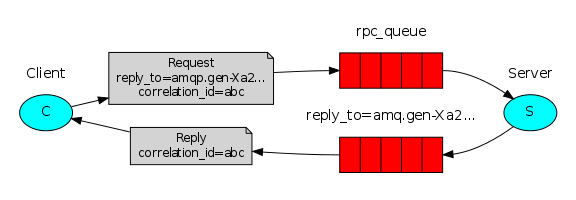
\includegraphics[width=\textwidth]{rpc.png}
    \end{figure}
\end{frame}

\section{Интеграция с World Of Tanks}
\begin{frame}{ДВА МИРА}
    \begin{columns}

    \begin{column}{0.33\textwidth}
    \begin{block}{World of Tanks}
        \begin{itemize}
            \item специальный движок
            \item распределённый
            \item высоконагруженный
        \end{itemize}
    \end{block}
    \end{column}
     
    \begin{column}{0.33\textwidth}
    \begin{block}{LAMP}
        \begin{itemize}
            \item просто
            \item стабильно
            \item огромный опыт
        \end{itemize}
    \end{block}
    \end{column}

    \begin{column}{0.33\textwidth}
    \begin{block}{Цель}
        \begin{itemize}
            \item независимость
            \item доступность
            \item минимизация рисков
        \end{itemize}
    \end{block}
    \end{column}

    \end{columns}
\end{frame}

\begin{frame}{ЭКСПОРТ ДАННЫХ}
    \begin{block}{BigWorld}
        \begin{itemize}
            \item{аккаунты}
            \item{кланы}
            \item{результаты боёв}
        \end{itemize}
    \end{block}

    \begin{block}{AMQP}
        \begin{itemize}
            \item{RabbitMQ}
            \item{доработка движка}
        \end{itemize}
    \end{block}
\end{frame}

\begin{frame}{УПРАВЛЕНИЕМ ИЗ ВНЕ}
    \begin{block}{Сервер}
        \begin{itemize}
            \item управление аккаунтом
            \item управление кланом
            \item создание боёв
        \end{itemize}
    \end{block}

    \begin{block}{AMQP}
        \begin{itemize}
            \item асинхронный подход
        \end{itemize}
    \end{block}
\end{frame}

\section{Поддержка множества игр}
\begin{frame}{АУТЕНТИФИКАЦИЯ}
    \begin{itemize}
        \item аутентификация - проверка личности
        \item авторизация - проверка прав
        \item внешний сервис аутентификации
    \end{itemize}
\end{frame}

\begin{frame}{WARGAMING ID}
    \begin{itemize}
        \item OpenID
        \item внутренний и внешний API
        \item расширение для единого выхода
    \end{itemize}
\end{frame}

\begin{frame}{НАСТОЯЩЕЕ И БУДУЩЕЕ}
    \begin{itemize}
        \item ранняя интеграция игр
        \item lazy-регистрация
        \item единый премиум
        \item ...
    \end{itemize}
\end{frame}

\section{Заключение}
{
\usebackgroundtemplate{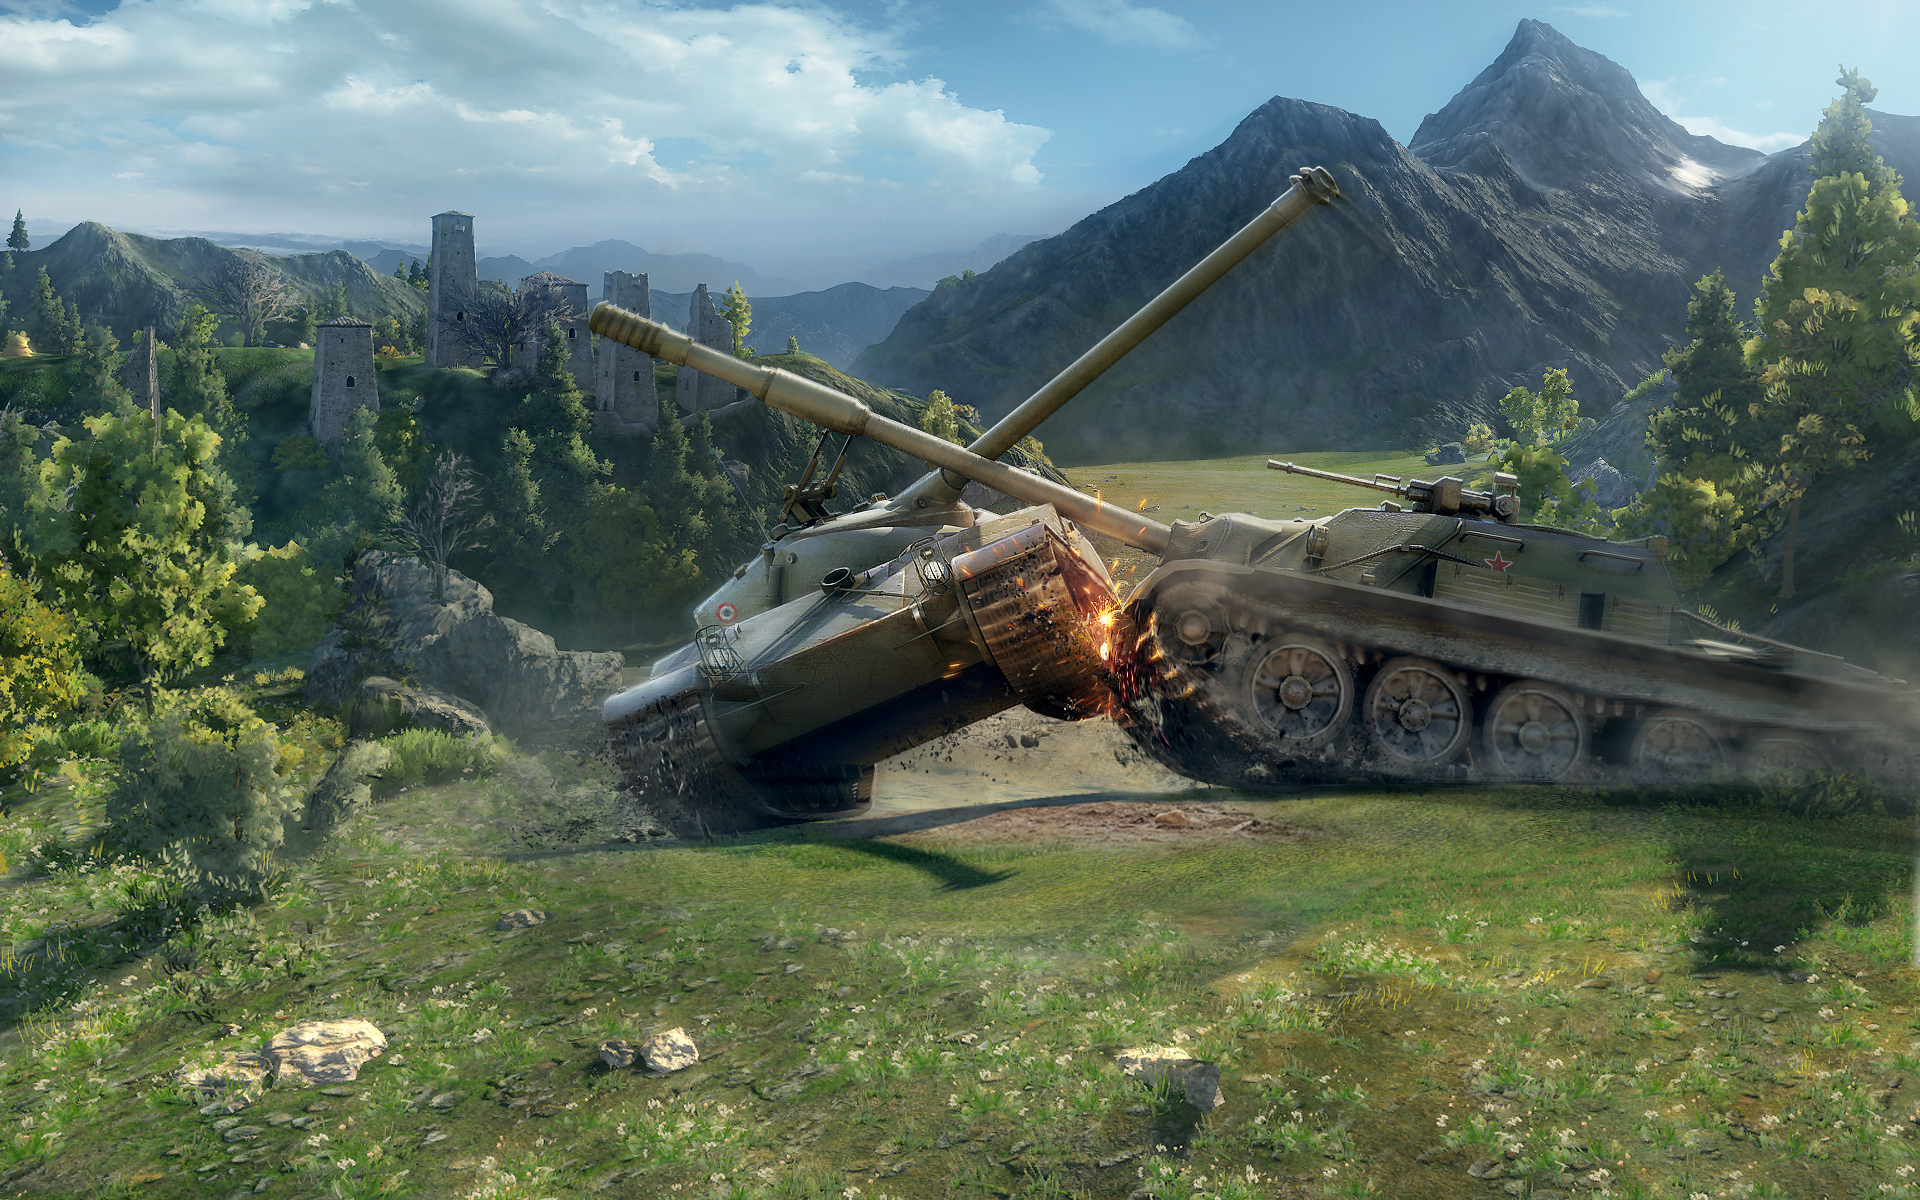
\includegraphics[width=\paperwidth]{wot.jpg}}
\begin{frame}[plain]{}
\end{frame}
}

\begin{frame}{ИДЕИ}
    \begin{itemize}
        \item главное --- скорость и простота разработки
        \item не стоит боятся гетерогенной среды
        \item синхронный подход везде где можно
        \item асинхронный --- только там, где это необходимо
        \item AMQP --- отличный протокол для реализации RPC
    \end{itemize}
\end{frame}

{
\setbeamertemplate{footline}{}

\setbeamercolor{frametitle}{fg=white}
\setbeamercolor{normal text}{fg=white}
\setbeamercolor{block title}{fg=white}
\setbeamercolor{block body}{fg=red}

\usebackgroundtemplate{
\includegraphics[height=\paperheight]{wg-end.jpg}}
\begin{frame}{СПАСИБО ЗА ВНИМАНИЕ. ВОПРОСЫ}
    \begin{block}{Максим Мельников}
    \par \url{mailto:m\_melnikau@wargaming.net}
    \par \url{https://plus.google.com/114669104565190507739/}
    \par \url{https://twitter.com/max\_posedon}
    \par \url{http://wargaming.com}
    \end{block}
\end{frame}
}

\end{document}

